\chapter{数据库设计}
\section{数据库环境说明}
本系统的数据系统采用Oracle数据库系统。


\section{数据库的命名规则}
是否允许单词缩写,允许的单词缩写有哪些。

表名是单数还是复数。关联表如何命名。字符数限制等。

字段是否带上前缀(如integer类型则加上i前缀等)。

\section{逻辑设计}
数据库应达到3NF范式。以新奥尔良方法为基础,基于ER模型和关系模式进行数据库设计。

概念设计:基于ER模型。

逻辑设计:基于关系模式设计。

采用的计算机辅助设计工具:PowerDesigner(SYBASE)。

\subsection{ER模型要素}

\subsubsection{实体}
本应用数据库中涉及到的实体有:考生、考试、试卷。

\subsubsection{联系}
实体与实体间的联系有:

1、考生与考试间的报名关系,是一个多对多的关系。

2、考生与考试间的参加关系,是一个多对多的关系。

3、考试与试卷间的使用关系,是一个多对一的关系。

\subsubsection{确定实体属性}
考生具有的属性有:姓名、性别、生日、证件号、地区、邮寄地址、联系方式。其中证件号是主码。

考试具有的属性有:时间、地点。(时间,地点)是主码。

试卷具有的属性有:试卷编号,题1编号,...,题100编号。试卷编号是主码。

\subsubsection{确定联系属性}
考生和考试间的参加关系具有“成绩”属性。

\section{示例}
\begin{figure}[ht]
\centering
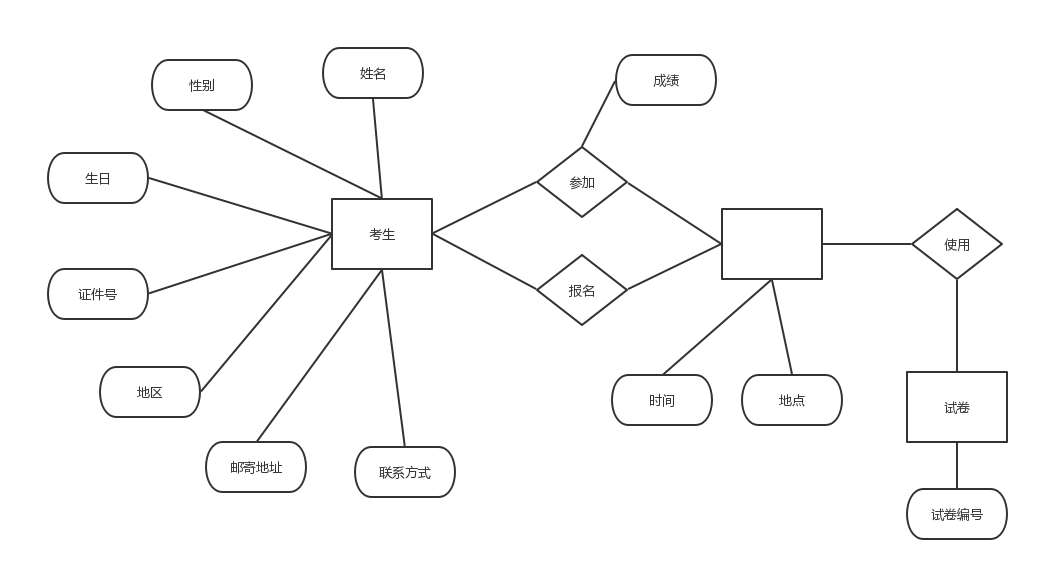
\includegraphics[width=16cm]{ER.png}
\caption{ER图} \label{fig:figure1}
\end{figure}



\section{物理设计}

\subsection{数据库产品}
使用 Oracle Database 12c 企业版,采用集中式的数据库。

\subsection{实体属性、类型、精度}
考生、考试、试卷三个实体各自转换成一个关系模式。除此以外,由于考生与考试间的报名关系、考生与考试间的参加关系是多对多的关系,因此也要各转换成一个关系模式。

ETS管理员并不是需要存储在数据库中的实体。

\subsubsection{考生数据表Examinee设计}
\begin{table}[htbp]
\centering
\caption{考生数据表Examinee设计} \label{tab:client-database}
\begin{tabular}{|c|c|c|c|c|}
    \hline
    字段名 & 类型 & 大小 & 说明 & 备注 \\
    \hline
    name & char & 20 & 用户的英文姓名 & · \\
    \hline
    sex & char & 1 & 用户的性别 & · \\
    \hline
    date of birth & date & · & 用户的生日 & · \\
    \hline
    ID & char & 64 & 用户的证件号 & 主码 \\
    \hline
    location & char & 200 & 用户所在地区(大范围) & · \\
    \hline
    mail address & char & 200 & 用户希望的成绩单邮寄地址 & · \\
    \hline
    contact & char & 11 & 用户的手机号或电话号 & · \\
    \hline
\end{tabular}
\note{考生数据表Examinee设计}
\end{table}

\subsubsection{考试数据表Exam设计}
记录未来12月将举办的考试的时间、考点与考位信息。
\begin{table}[htbp]
\centering
\caption{考试数据表Exam设计} \label{tab:order-database}
\begin{tabular}{|c|c|c|c|c|}
    \hline
    字段名 & 类型 & 大小 & 说明 & 备注 \\
    \hline
    time & date & · & 考试的日期 & 和centerNo一起构成主码 \\
    \hline
    centerNo & int & 4 & 举办考试的考点编号 & 和time一起构成主码 \\
    \hline
    quota & int & 4 & 剩余考位 & · \\
    \hline
\end{tabular}
\note{考试数据表Exam设计}
\end{table}

\subsubsection{试卷数据表设计}
试卷数据表中记录每份试卷的题目在题库中的编号。默认每份试卷有100题。每份试卷有唯一的编号,是整型。

\begin{table}[htbp]
\centering
\caption{试卷数据表TestPaper设计} \label{tab:order-database}
\begin{tabular}{|c|c|c|c|c|}
    \hline
    字段名 & 类型 & 大小 & 说明 & 备注 \\
    \hline
    paperNo & int & 4 & 试卷编号 & 主码 \\
    \hline
    Q1No & int & 4 & 第1题编号 & · \\
    \hline
    ... & ... & ... & ... & ... \\
    \hline
    Q100No & int & 4 & 第100题编号 & · \\
    \hline
\end{tabular}
\note{试卷数据表TestPaper设计}
\end{table}

\subsubsection{考试注册数据表Registration设计}
该表只记录尚未举行的考试的报名信息。
\begin{table}[htbp]
\centering
\caption{考试注册数据表Registration设计} \label{tab:order-database}
\begin{tabular}{|c|c|c|c|c|}
    \hline
    字段名 & 类型 & 大小 & 说明 & 备注 \\
    \hline
    examineeID & char & 64 & 考生的证件号 & 和centerNo一起构成主码 \\
    \hline
    examTime & date & · & 考试日期 & 和examineeID、centerNo一起构成主码 \\
    \hline
    centerNo & int & 4 & 举办考试的考点编号 & 和examineeID、examTime一起构成主码 \\
    \hline
\end{tabular}
\note{考试注册数据表Registration设计}
\end{table}

\subsubsection{考生考试成绩数据表Grades设计}
\begin{table}[htbp]
\centering
\caption{考生考试成绩数据表Grades设计} \label{tab:order-database}
\begin{tabular}{|c|c|c|c|c|}
    \hline
    字段名 & 类型 & 大小 & 说明 & 备注 \\
    \hline
    examineeID & char & 64 & 考生的证件号 & 和examTime、centerNo一起构成主码,同时是外码 \\
    \hline
    examTime & date & · & 考试日期 & 和examineeID、centerNo一起构成主码,同时是外码 \\
    \hline
    centerNo & int & 4 & 举办考试的考点编号 & 和examineeID、examTime一起构成主码,同时是外码 \\
    \hline
    grade & int & 4 & 考生成绩 & · \\
    \hline
\end{tabular}
\note{考生考试成绩数据表Grades设计}
\end{table}



\section{安全性设计}
备份和容灾设计。

服务器中的数据需定期备份。其中,考生用户的数据每小时备份一次,考试注册信息每小时备份一次。试卷与题库数据在每次更新时备份一次,考生成绩数据在每举行一次考试以及出分时各备份一次。考试信息一般不发生变化,因此除非有更新,否则一个月备份一次。

服务器必须安装不间断电源以防止停电或电压不稳造成的数据丢失的损失。若真断电时,在断电恢复过程可采用Oracle的日志文件,对其进行ROLLBACK处理,对数据进行恢复。

此外,服务器应在多个地方有冗余存储,如在多个城市建立数据中心进行数据的冗余备份,以防遭受人为或自然的破坏。

\section{数据库管理与维护说明}
对于数据库的维护,随时对数据库中的信息加以调试和保存备份。同样需要个工作人员进行系统的分析和用户的反馈,对系统进行升级以及功能的完善。同时保证系统安全有序的运行。

数据库的维护工作由ETS的专门管理人员完成。主要的维护工作有:

1、为各个数据表建立适当的索引以加快查询

2、定期(一般为一个月)发布新的考试信息

3、发布新试题时更新testPaper数据表信息

4、在每次考试后,将数据从Registration表中迁移到Grades表中,并加上考生成绩属性

5、定期(一般为一个月)将数据备份至永久存储介质(如磁带等)

6、对各类用户授予合适的权限

6、为数据建立完整性约束,如类型约束、引用完整性约束等。